\documentclass[10pt]{beamer}

\usetheme{metropolis}

%\setsansfont{default}
%\setmonofont{default}
%\usebeamerfont*{default}
%\setmonofont{Fira Mono}
%\setmathfont{TeX Gyre Pagella Math}[Scale=MatchLowercase] 
%\setsansfont{Latin Modern Sans}

\usepackage[ngerman]{babel}

\usepackage[utf8]{inputenc}

\usepackage[backend=biber,style=authortitle-ibid
  %,maxcitenames=1,ibidpage=true
]{biblatex}

\AtEveryCitekey{\clearfield{doi}}
\AtEveryCitekey{
  \clearfield{urlyear}
  \clearfield{urlmonth}
  \clearfield{language}
  \clearfield{origlanguage}
}
\AtEveryBibitem{
  \clearfield{language}
}

\renewbibmacro*{cite:ibid}{\printtext[bibhyperref]{\bibstring[\mkibid]{ibidem}}} 
\bibliography{pres}

\usepackage{chemformula}

\usepackage[normalem]{ulem}

\usepackage{appendixnumberbeamer}
\usepackage{booktabs}
\usepackage[scale=2]{ccicons}

\usepackage{pgfplots}
\usepgfplotslibrary{dateplot}

\usepackage{amsmath}
\usepackage{mathtools}
\usepackage{algorithm}
\usepackage[noend]{algpseudocode}

\usepackage{xmpmulti}


\let\Footnotesize=\footnotesize  % save the definition
\let\footnotesize=\tiny  % make a footnotesize change very visible

\usepackage{xspace}
\newcommand{\themename}{\textbf{\textsc{metropolis}}\xspace}

\title{Die Abhängigkeit von den Autokratien}
\subtitle{Brauchen wir (russisches) Erdgas? Ist Erdgas nachhaltig?}
\date{17. Juni 2022}
\author{Marius Hegele}
\institute{Technik und Fortschritt im Anthropozän, SoSe 2022, ZAK/KIT}
% \titlegraphic{\hfill\includegraphics[height=1.5cm]{logo.pdf}}

\begin{document}

\maketitle

\begin{frame}{Motivation}

  \settowidth{\leftmargini}{\usebeamertemplate{itemize item}}
  \addtolength{\leftmargini}{\labelsep}

  \small{
  \begin{itemize}
    \item Deutschland bezieht \textbf{500 TWh/a} = 55\% des Gesamtgasbedarfs aus Russland (2020)\footfullcite{clausen2022}
    \item umgekehrt machen Exporte nach DE 25\% der russischen Gasexporte aus\footfullcite{iwd}
    \item Deutsche Erdgasspeicher Stand 05.03. nur zu 27\% gefüllt (normal 50-80\%)\footcite{leo}
      % erheblicher Teil über Konzernbeteiligung von Gazprom kontrolliert
    \item 30.03: BMWK ruft Frühwarnstufe des Notfallplans Gas aus\footfullcite{bmwk}
      % jeder Verbraucher ist angehalten seinen Verbrauch so gut wie möglich zu reduzieren
    % \item Russland droht mit Gaslieferstopp, akzeptiert die Bezahlung nur noch in Rubel\footcite{bmwk}
    \item 15.06: Gazprom schickt nur noch 0.7 statt 1.7 TWh/d (-59\%) durch Nord Stream Leitung (Reparaturarbeiten)\footfullcite{gazprom-gasverknappung}
  \end{itemize}
  }
\end{frame}

\part{Brauchen wir (russisches) Erdgas?}
\frame{\partpage}

\begin{frame}{Teil I: Brauchen wir (russisches) Erdgas?}
  \setbeamertemplate{section in toc}[sections numbered]
  \tableofcontents[hideallsubsections,part=1]
\end{frame}


\section{Direkter Ersatz durch Importe}

\begin{frame}
\begin{columns}
\column{0.7\textwidth}
\includegraphics[height=0.95\textheight]{fig/erdgasreserven.png}
\column{0.3\textwidth}
\centering
\scriptsize{\fullcite{statista-erdgasreserven}}
\end{columns}
\end{frame}

\begin{frame}{Abhängigkeit von Autokratien}
  ``Der Fluch der Rohstoffe'' / ``Paradox of Plenty''

  Reichtum an Rohstoffen = Demokratiedefizit, extreme Korruption, Entwicklungshemmnis

  Rohstoffe (Energieträger, industrielle Rohstoffe, Minerale, \dots) als bedeutende Einnahmequellen für Eliten:
  Gewinne fließen nicht in die Entwicklung, sondern in die Aufrechterterhaltung der Herrschaft

  Instabilität und kriegerische Auseinandersetzung über Kontrolle der Rohstoffe

  \smallskip
  \scriptsize{\fullcite{gabler}}
\end{frame}


\begin{frame}{Pipelineimporte}
\begin{columns}
\column{0.7\textwidth}
\includegraphics[width=\textwidth]{fig/gaspipelines.png}
\scriptsize{\fullcite{gaspipelines}}
\column{0.3\textwidth}
Erhöhung Importe aus Aserbaidschan, Norwegen 2022 um 106 TWh EU-weit möglich.

\centering
\smallskip
\scriptsize{\fullcite{iea2022}}
\end{columns}
\end{frame}

\begin{frame}{Flüssiggasimporte}

\settowidth{\leftmargini}{\usebeamertemplate{itemize item}}
\addtolength{\leftmargini}{\labelsep}

\begin{columns}
\column{0.6\textwidth}
\includegraphics[width=\textwidth]{fig/gasnetz-europa.png}
\scriptsize{\fullcite{ei1}}
\column{0.4\textwidth}
\small{
\begin{itemize}
\item Herkunft primär: USA, Australien, Katar\footnotemark
\item in naher Zukunft realistisch 212 TWh EU-weit möglich\footnotemark
\item EU-27: LNG-Terminal Kapazität 1100 TWh für Importe aus anderen Ländern\footnotemark
  + Türkei\footnotemark
\item LNG-Beschleunigungsgesetz: 11 LNG-Terminals für Deutschland = 286 TWh\footnotemark
\end{itemize}
}
\end{columns}
\smallskip
\footnotetext[5]{\fullcite{leo}}
\footnotetext[6]{\fullcite{iea2022}}
\footnotetext[7]{\fullcite{iwd}}
\footnotetext[8]{\fullcite{leo}}
\footnotetext[9]{\fullcite{lng-gesetz}}
\end{frame}

% Nachhaltigkeit LNG-Gas (schlimmer als Erdgas?)

\begin{frame}{Flüssiggas: Probleme}
  \begin{itemize}
\item Bottleneck: Weiterverteilung über Gasnetz (insb. v. Spanien) \footfullcite{iwd}
\item Energieintensive Umwandlung, Transport, Wiederaufbereitung 
  \\ $\Rightarrow$ deutlich teurer, höhere Emissionen \footfullcite{lng-faq}
\item Große Investition nicht sinnvoll, mittelfristig: Klimaneutralität
% \item Schiefergas (Fracking): Grundwasserverschmutzung
  \end{itemize}
\end{frame}

\section{Ansätze im Verbrauch}

\begin{frame}
% zweitwichtigster Energieträger
% \begin{figure}
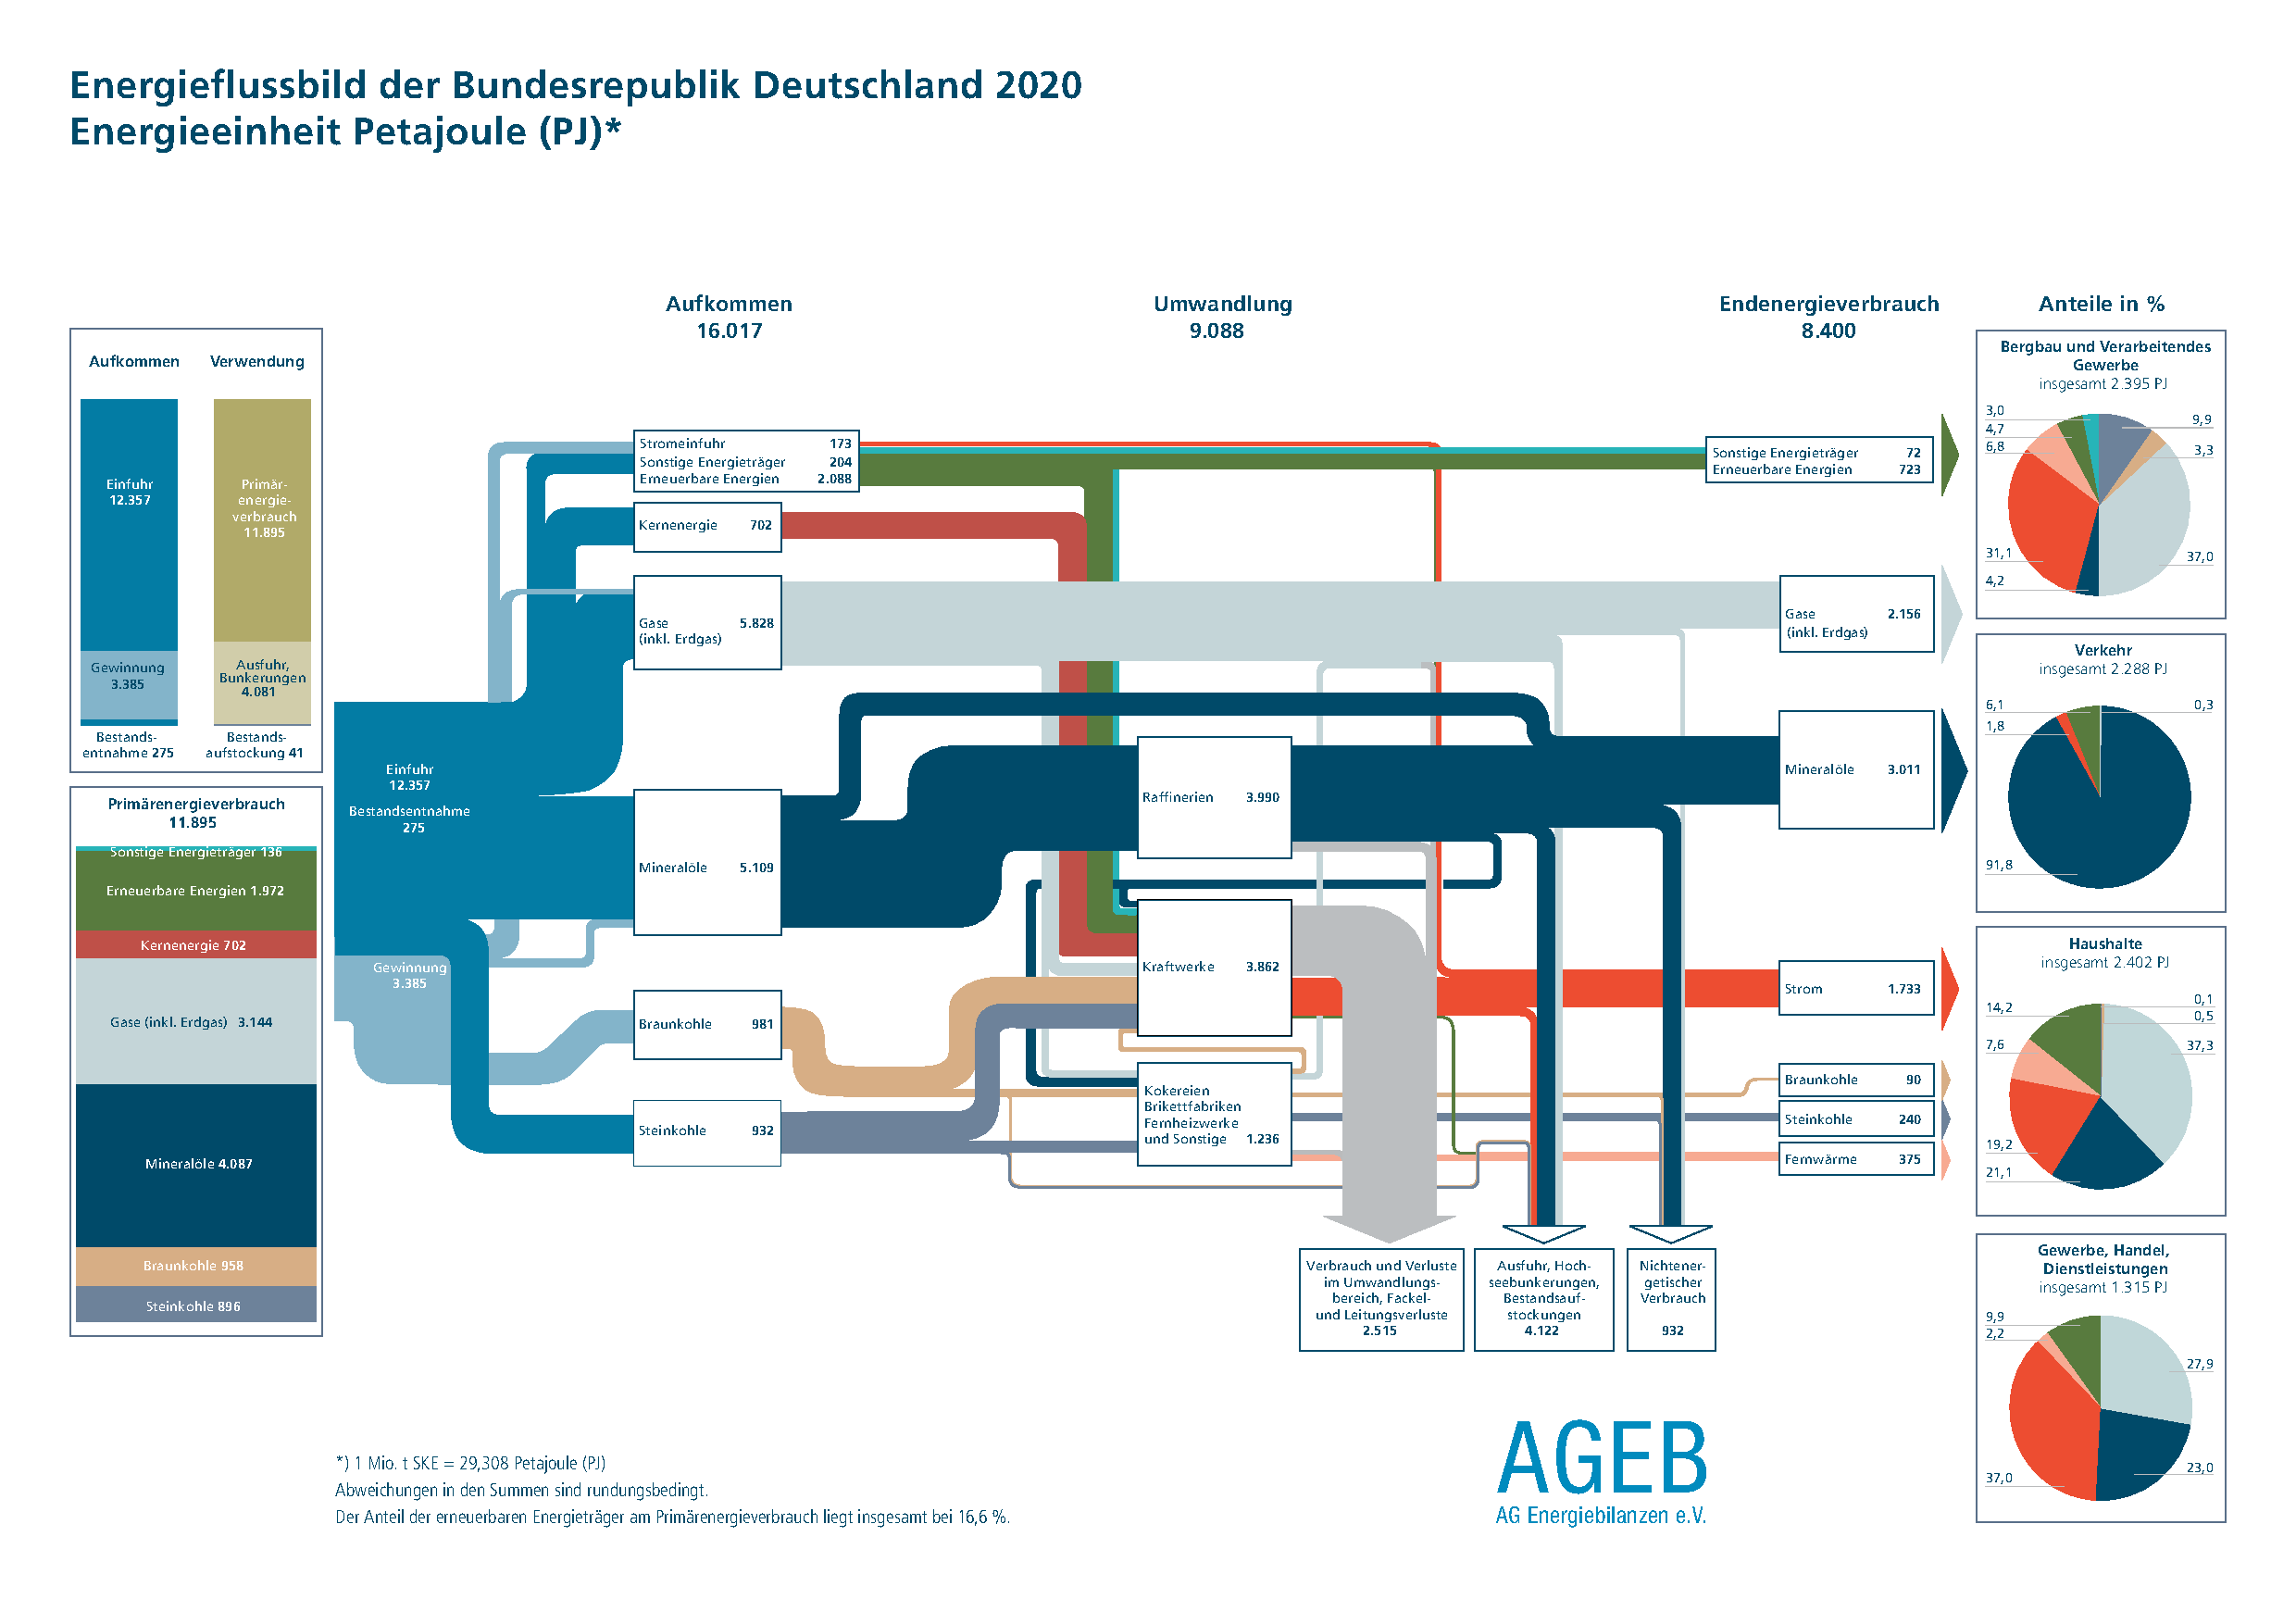
\includegraphics[width=1.1\textwidth]{fig/Energieflussbild-2020_PJ_lang_DE_20220401}

% \scriptsize{\fullcite{energieflussbild}}
% \end{figure}
\end{frame}

\begin{frame}{Gasspeicher regulieren}
  \begin{itemize}
    \item 265 TWh Kapazität in Deutschland \footfullcite{iwd}
    \item Russland kontrolliert über Konzerbeteiligung erheblichen Teil der Speicher
    \item Stattdessen öffentliche Regulierung, 
      auch da volle Gasspeicher ökonomische Risiken für Privateigentümer bergen \footfullcite{leo}
  \end{itemize}
\end{frame}

\section{Raum- und Prozesswärme}

\begin{frame}
Insgesamt 598 TWh/a (66\%) Erdgas. 49,5\% der Heizungen sind Gasheizungen.

\begin{figure}
\includegraphics[width=0.9\textwidth]{fig/einsatz_erdgas.png}

\scriptsize{\fullcite{clausen2022}}
\end{figure}
\end{frame}

% \begin{frame}{Effizienz}
%   \begin{figure}
%   \includegraphics[height=0.6\textheight]{fig/einsparpotential.png}
%   \end{figure}
%   \scriptsize{\fullcite{janson2022}}
% \end{frame}

\begin{frame}{Kurzfristiges Wärmeeinsparpotential}
  \small{
  \begin{itemize}
    \item Wohnung: Reduktion um 1 Grad EU-weit = Reduktion des Erdgasverbrauchs um 100 TWh/a \footfullcite{iea2022}
    \item automatisch: Einsparungen durch sowieso schon hohe Preise  \\
      $\Rightarrow$ keine Steuersenkungen oder andere Subventionen (stattdessen Energiegeld) \footfullcite{clausen2022}
    \item Intelligentes Heizen: Vernetzte Thermostatventile, Heizungssteuerungen: Welche Räume wann und wie heizen? \footcite{clausen2022}
    % \item Regularien entwickeln, sodass sich (nur langfristig rentable) Energiesparmaßnahmen
    %   betriebswirtschaftlich rechnen \footcite{clausen2022}
    %   % (Reduzierung der gesetzlichen Abschreibungsfristen) 
    \item Sanierungen: standardisierte Upgrades (Isolation) \footfullcite{iea2022}
  \end{itemize}
  }
\end{frame}

\begin{frame}{Langfristiger Ersatz im Wärmesektor}
 \begin{itemize} 
    \item Anschluss an Wärmenetze
    \item Elektrifizierung über Wärmepumpen (langfristig 60-70\% des Wärmebedarfs) \footfullcite{clausen2022}
    \item Regenerative Wärmequellen: Solarthermie, Geothermie, (Abfallverbrennung, Biomasse)
      (mit Erdbecken-Wärmespeicher) \footcite{clausen2022}
    \item (Wasserstoff in dezentralen (Gas-)Heizungen)\footcite{clausen2022}
    \item Effiziente Wärmeverteilung durch effiziente Pumpen \footfullcite{ei1}
 \end{itemize}
 % Block-Heizkraftwerke?
 % Tangierend notwendige Maßnahmen: Fachkräfteinitative Wärmepumpeninstallation, 
 %  Förderung von Erdgas-Brennwertheizungen beenden / verbieten,
 %  finanzielle Anreize, Förderprogramme
\end{frame}

\begin{frame}{Anschluss an Wärmenetze}
\begin{figure}
\includegraphics[width=\textwidth]{fig/kraft-waerme-kopplung.jpg}

\scriptsize{\fullcite{kwk}}
\end{figure}
\end{frame}


\begin{frame}{Elektrifizierung über Wärmepumpen}
\begin{figure}
\includegraphics[width=\textwidth]{fig/waermepumpe.png}

\scriptsize{\fullcite{ei1}}
\end{figure}
\end{frame}


\section{Strom}

\begin{frame}[label=gas-eff]
\begin{figure}
\includegraphics[width=\textwidth]{fig/efficiency_power_plants.png}

\scriptsize{\fullcite{ei1}}
\end{figure}
\end{frame}

\begin{frame}[label=gas-co2]
\begin{figure}
\includegraphics[width=\textwidth]{fig/co2_emissions_power_plants.pdf}

\scriptsize{\fullcite{uba-co2}}
\end{figure}
\end{frame}

\begin{frame}[label=gas-flex]
\begin{columns}
\column{0.7\textwidth}
\includegraphics[width=\textwidth]{fig/flexibility_power_plants.png}
\column{0.3\textwidth}
\includegraphics[width=\textwidth]{fig/net_power.png}
\includegraphics[width=\textwidth]{fig/ramp_rate.png}
\end{columns}
\scriptsize{\fullcite{agora}}
\end{frame}


\begin{frame}{Stromproduktion: Erdgasersatz}
  \small{
  171/a TWh Erdgas zur Produktion von 95 TWh/a Elektrizität

  \begin{itemize}
    \item Kurzfristig: Kohle oder Öl können große Mengen schnell ersetzen: 
      296 TWh EU-weit ohne Mehremissionen \footfullcite{iea2022}
    \item Emissionen durch Emissionshandel fest begrenzt: 
      Einsparung an anderer Stelle $\Rightarrow$ Preissteigerung \footfullcite{leo}
    \item Atomkraft: Verlängerung des vorbereiteten Laufzeitendes 
      technisch herausfordernd und ökonomisch aufwendig \footcite{leo}
    \item Erneuerbare Energien: 
      45 TWh = 40\% der bisher installierten Kapazität 
      $\Rightarrow$ Flächenausweisung, Verfahren vereinfachen, Förderprogramme \footcite{leo}
    \item Ersatz für Gas als Flexibilitätsquelle (Frequenzstablitätsregelung):
      Kurz- und Langfristspeicher, Demand Side Management \footcite{iea2022}
      % Spitzenlastabdeeckung, demand shifting, peak shaving, schnelle Regelbarkeit
  \end{itemize}
  }
\end{frame}

\section{Chemieindustrie}

\begin{frame}
\begin{figure}
\includegraphics[width=0.9\textwidth]{fig/anteile_chemieindustrie.png}

\scriptsize{\fullcite{vci2022}}
\end{figure}
\end{frame}


\begin{frame}
  \begin{columns}
  \column{0.8\textwidth}
  \only<2>{
  Beispiel Ammoniakherstellung: 99\% nach Haber-Bosch Verfahren\footnotemark:

  \begin{scriptsize}
    \begin{itemize}
      \item Dampfreformierung: Methan + Wasser + Energie $\Rightarrow$ Wasserstoff
      \item Stickstoff + Wasserstoff + Prozesswärme (Erdgas) $\Rightarrow$ Ammoniak
    \end{itemize}
  \end{scriptsize}

  Verwendung: größtenteils Düngemittelproduktion
  }
  \column{0.2\textwidth}
  \includegraphics[width=0.9\textwidth]{fig/campus_hochdruck_reaktor.png}
  \end{columns}
  \only<2>{\footnotetext[25]{\fullcite{smil}}}
\end{frame}

\begin{frame}{Wasserstoffproduktion ohne Erdgas}
  \begin{small}
  Elektrolyse: Wasser + Strom $\Rightarrow$ Wasserstoff + Sauerstoff

  aktuell: nur Pilotanlagen, bis 2030 nur geringe Kapazität, bleibt teuer (100 EUR pro MWh -- Erdgas 40 EUR)\footfullcite{rnd}
  \end{small}

  % H2-Ready-Konzept: Gasnetze und -kraftwerke sollen auf Wasserstoff umstellbar sein

  \begin{figure}
    \includegraphics[width=0.55\textwidth]{fig/wasserstoff-strombedarf.png}

    \scriptsize{\fullcite{agora-wasserstoff}}
  \end{figure}
\end{frame}



\part{Ist Erdgas nachhaltig?}
\frame{\partpage}

\begin{frame}{Teil II: Ist Erdgas nachhaltig?}
  \setbeamertemplate{section in toc}[sections numbered]
  \tableofcontents[hideallsubsections,part=2]
\end{frame}

\section{EU-Taxonomie}


\begin{frame}{EU Verordnung: Taxonomie für nachhaltige Entwicklung}
  \small
  \begin{itemize}
    \item Rahmenbedingungen für Investitionen: was ist nachhaltig? \footfullcite{reuters}
    \item Ziel: private Investitionen in Tätigkeiten mobilisieren, die notwendig sind um die Klimaneutralität zu erreichen \footfullcite{eu-komm}
    \item 31.12.21 Beschlussentwurf der EU-Kommision: 
      (Atom- und) Gaskraftwerke sind unter folgenden Kriterien grün \footfullcite{taz-taxonomie}
    \begin{itemize}
      \item Muss fossile Altanlage ersetzen \footcite{taz-taxonomie}
      \item Maximal 270 g/kWh direkte Emissionen oder 550 g/kW durchschnittliche Emissionen über 20 Jahre \footfullcite{uba}
        % $\Rightarrow 1,4 \cdot 10^9$ tCO2e nachhaltig, wenn alle Kohlekraftwerke durch Gaskraftwerke ersetzt werden
    \end{itemize}
  \end{itemize}
\end{frame}

\begin{frame}
\begin{figure}
\includegraphics[width=\textwidth]{fig/headline-taxonomie.png}

\scriptsize{\fullcite{spiegel-taxonomie}}
\end{figure}
\end{frame}

\section{Pro}

\againframe{gas-eff}
\againframe{gas-co2}
\againframe{gas-flex}

\begin{frame}{Pro: Erdgas als nachhaltig klassifizieren}
    Ersatz beim Kohleausstieg \footfullcite{reuters}:
    Stabilitätsreserve und Flexibilitätsquelle im Übergang zu EE-Stromproduktion \footfullcite{eu-komm}
\end{frame}

\section{Contra}

\begin{frame}
  \begin{itemize}
    \item Leckage in Pipelines\footfullcite{reuters}, Methan als kurzfristig sehr potentes Treibhausgas (25 CO2e)\footfullcite{uba-co2e}
    \item Setzt falsche Anreize: Gaskraftwerke anstatt EE\footfullcite{uba}
    \item Verstößt gegen den Grundsatz der Technologieneutralität: für andere gelten maximal 100 gCO2e/kWh\footcite{uba}
    % \item Taxonomie-Konformität schwer zu prüfen: Unsicherheit bei Investition\footcite{uba}
    \item Gefährdet Bedeutung und Glaubwürdigkeit der Taxonomie\footfullcite{dnr}
  \end{itemize}
\end{frame}

\begin{frame}{Ersatzvorschlag}
  Stattdessen\footfullcite{uba}
  \begin{itemize}
    \item separat regulieren
    \item jährliche Grenzwerte mit abnehmendem Verlauf
    \item Kriterien für kohlenstoffarme Gase definieren
  \end{itemize}
\end{frame}

\section{Süddeutsche Erdgasleitung}


\begin{frame}
\begin{figure}
\includegraphics[width=\textwidth]{fig/sel.png}

\scriptsize{\fullcite{terranets}}
\end{figure}
\end{frame}

\begin{frame}
  \begin{itemize}
    \item 250 km Gasleitung
    \item Gasbedarf wird in BW von 39,5 GW 2022 auf 49,1 GW 2030 wachsen, um Ausstieg aus Atom und Kohle abzusichern
    \item ist 2035 als erste Pipeline bereit, Wasserstoff nach BW zu transportieren
  \end{itemize}

  \centering
  \fullcite{terranets}
\end{frame}

\begin{frame}{Gasinfrastuktur ausbauen: sinnvoll?}
  Zukunft: Wasserstoff als Langzeitspeicher und industriell benötigter Stoff

  Drei Optionen: Beimischen (5-20\%), Wasserstoff methanisieren, reines Wasserstoffnetz\footfullcite{iis}

  Elektrolyse + Methanisierung effizient möglich und kann CO2 binden (76~\% HELMETH-Verfahren)\footfullcite{helmeth}

  Vorteile\footcite{iis}: 
  \begin{itemize}
    \item Große Pipeline haben mit 24 GW achtfache Übertragungskapazität von Hochspannungsleitung
    \item Gasnetz hat hohe existierende Speicherkapazität (265 TWh)
  \end{itemize}
\end{frame}

\begin{frame}
\begin{figure}
\includegraphics[width=\textwidth]{fig/multimodal-energy-grid.png}

\scriptsize{\fullcite{multimodal-grids}}
\end{figure}
\end{frame}

\begin{frame}{Anregung zur Diskussion}
    \begin{itemize}
      \item Kurzfristig: Importersatz durch LNG, wenn auch schwierig, teurer und nicht nachhaltig  
      \item Einsparungen über Kraft-Wärme-Kopplung, Sanierungen, intelligentes Heizen
      \item Teure Investitionen in Infrastruktur über die nächsten Jahrzehnte: Erneuerbare Energien, Wärmepumpen, Batterien, Wasserstoff
      \item Hand in Hand mit der Transformation zur Klimaneutralität 
      \item Einschränkung: Stabilität Stromnetz -- Gaskraftwerke als Enabler für PV und Wind
      \item Gas nicht nachhaltig, die dafür gebaute Infrastruktur schon (Wasserstoff)
    \end{itemize}
\end{frame}

\begin{frame}[allowframebreaks]

  \printbibliography
  % \bibliographystyle{abbrv}

\end{frame}

\end{document}